\documentclass{article}
\usepackage[a4paper]{geometry}
\usepackage[skip=10pt]{parskip}
\usepackage{amssymb}
\usepackage{graphicx}
\usepackage{hyperref}
\usepackage[section]{placeins}
\usepackage[official]{eurosym}
\usepackage{textgreek}
\usepackage{tcolorbox}
\usepackage{listings}
\usepackage{textcomp}
\usepackage{ccicons}
\usepackage{tikz}
\usepackage{multirow}
\usepackage{longtable}
\usepackage{wasysym}
\usepackage{nicefrac}
\usepackage{pdflscape}

\renewcommand{\familydefault}{\sfdefault}

\setlength\parindent{0pt}

\newenvironment{note}{\begin{tcolorbox}[colback=blue!5!white,colframe=blue!75!black,title=\textbf{Note}]}{\end{tcolorbox}}
\newenvironment{caution}{\begin{tcolorbox}[colback=red!5!white,colframe=red!75!black,title=\textbf{Caution}]}{\end{tcolorbox}}
\newcommand{\file}[1]{\texttt{#1}}

\lstset
{
	basicstyle=\footnotesize\ttfamily,
	breaklines=true,
	keywordstyle=\bfseries\color{green!40!black},
	commentstyle=\itshape\color{purple!40!black},
	identifierstyle=\color{blue},
	stringstyle=\color{orange},
	tabsize=4
}

\begin{document}
\hypersetup{pageanchor=false}
\begin{titlepage}
\thispagestyle{empty}
\centering
\textsf{\Huge MacroPad}\\[1cm]
\textsf{\Large Programmable USB Input Device}\\[3cm]
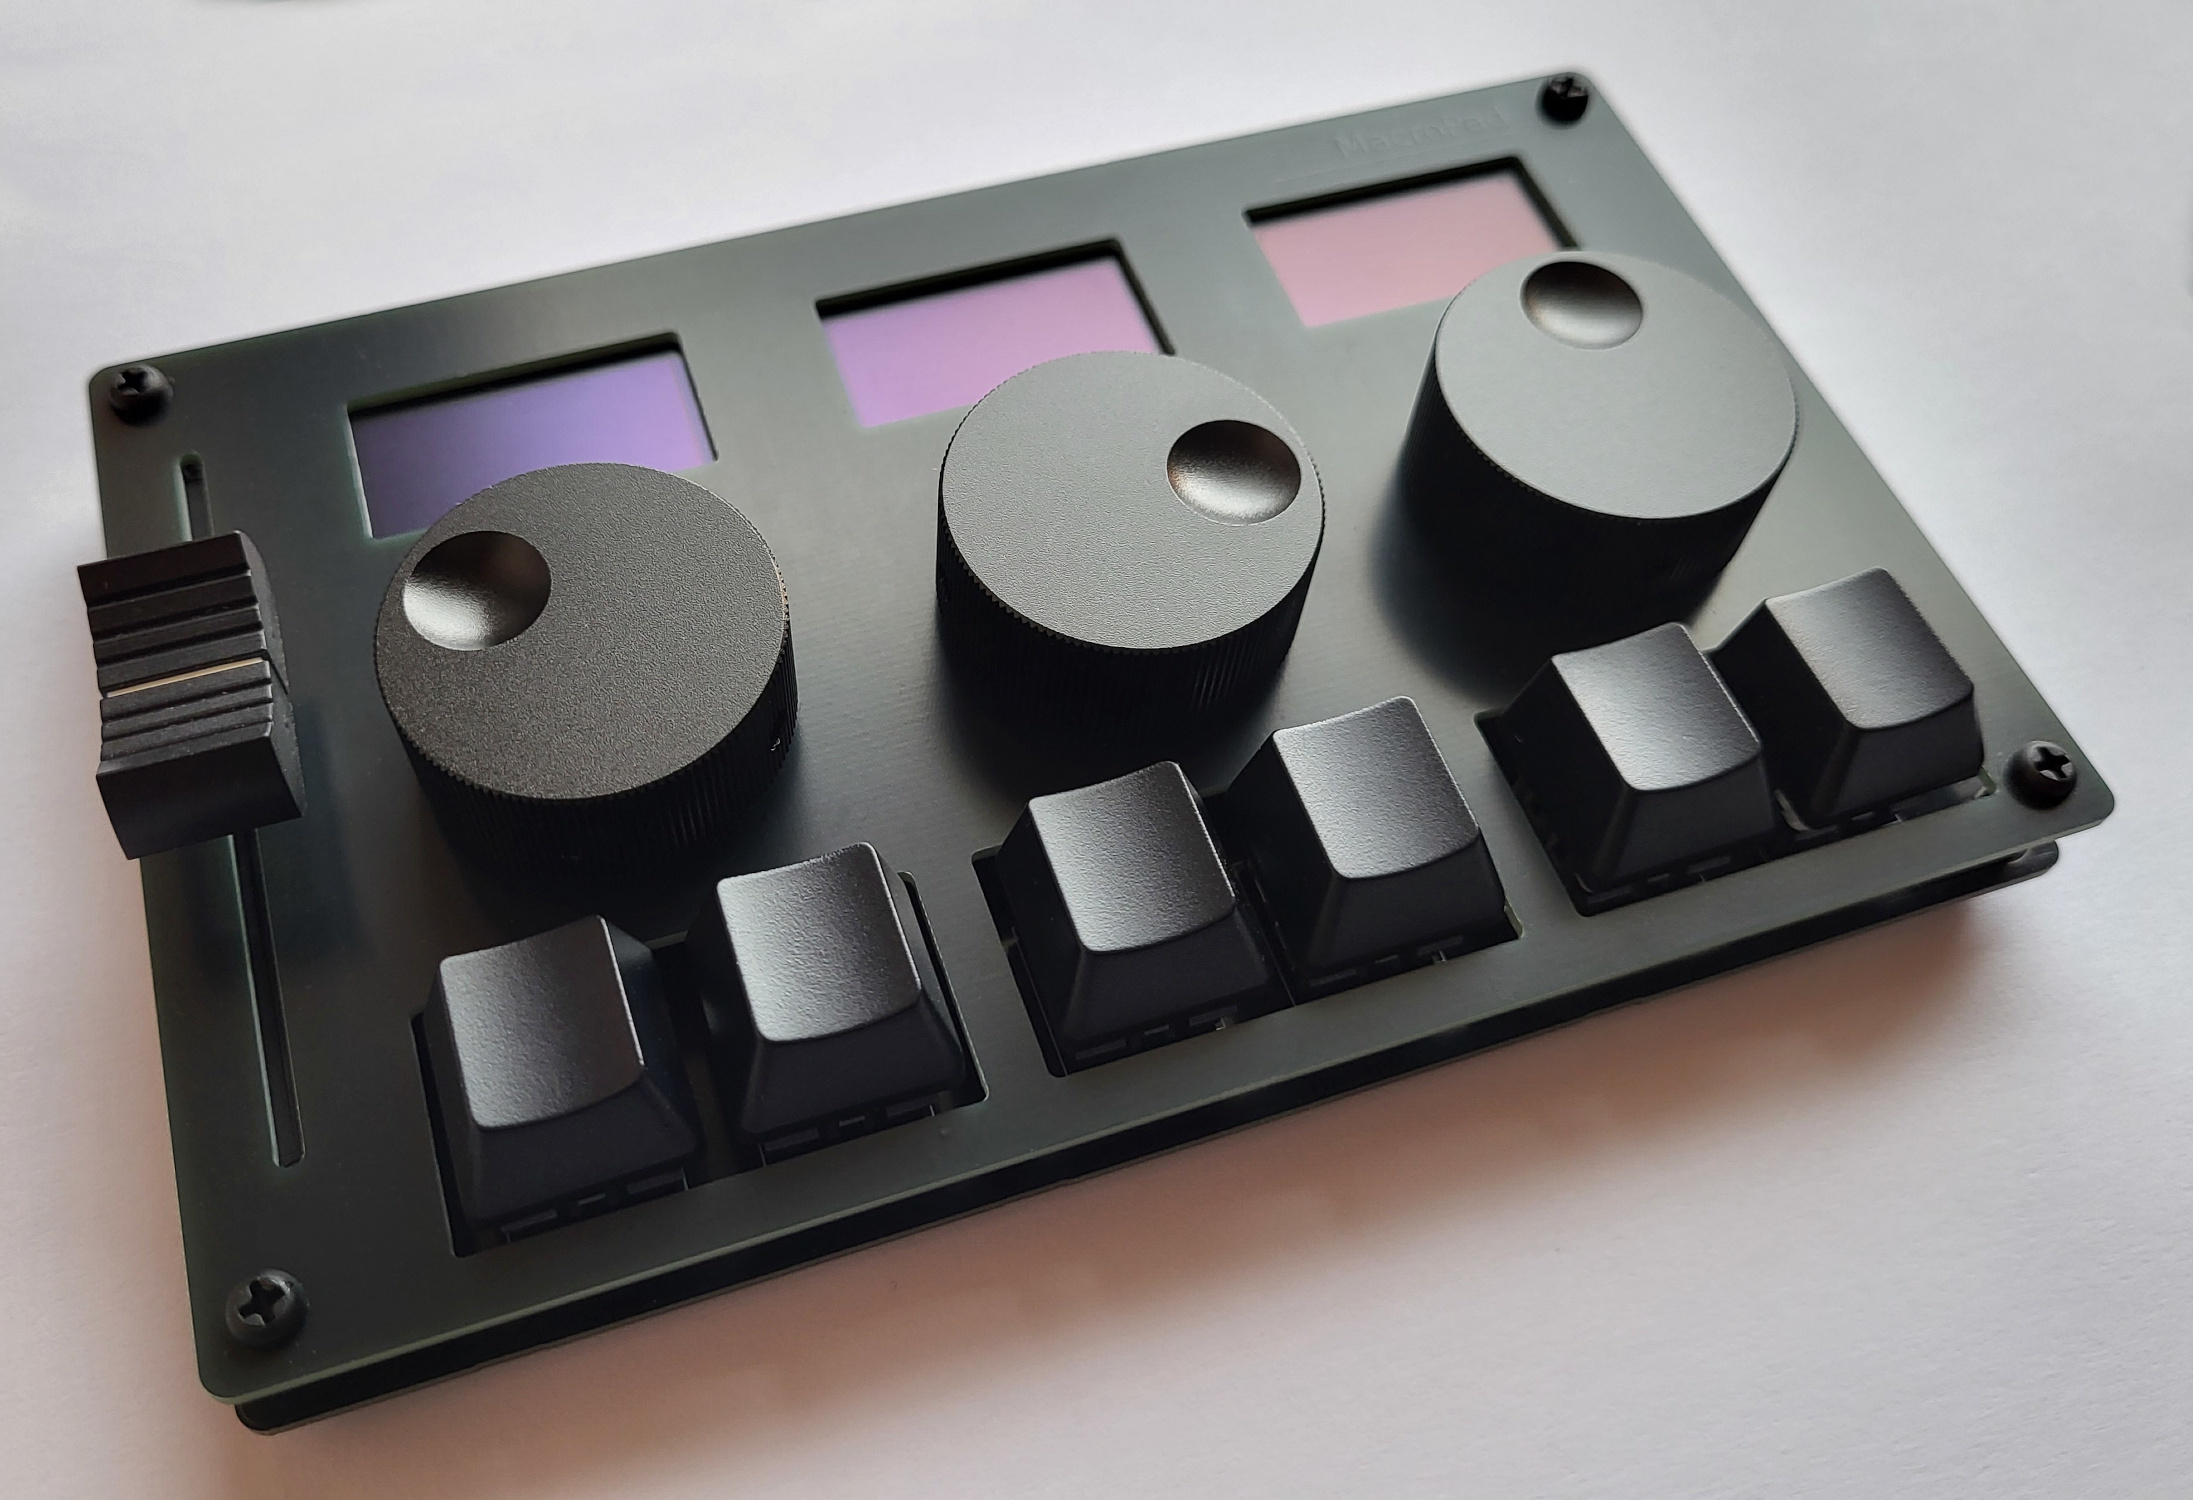
\includegraphics[width=\textwidth]{Images/Title.jpg}\\[3cm]
\textsf{\Large Building Instructions}
\end{titlepage}
\hypersetup{pageanchor=true}

\section*{License}
This document is licensed under Creative Commons \href{https://creativecommons.org/licenses/by-nc/4.0/}{Attribution-NonCommercial 4.0 International} (CC BY-NC 4.0 \ccCopy\,\ccAttribution\,\ccNonCommercial).

Attribution to \href{http://github.com/7vgn/MacroPad/}{http://github.com/7vgn/MacroPad/} is sufficient.

\tableofcontents

\section{Introduction}

\subsection{Cloning the GitHub Repository}\label{sec:gitclone}
The very first thing you should do is download (``clone'') the MacroPad GitHub repository to your computer. In order to do so, you first need to \href{https://git-scm.com/downloads}{install Git}.

Once installed, open a command prompt, navigate to the directory you want to download into, then run:
\begin{lstlisting}[language=bash]
git clone --recurse-submodules https://github.com/7vgn/MacroPad.git
\end{lstlisting}
This creates a subdirectory named \file{MacroPad} containing everything you need, including this document.
Downloading might take a few minutes since the \lstinline[language=bash]{--recurse-submodules} option also downloads other required libraries that are included as submodules. 

\subsection{How Much Does It Cost to Build One?}
Prices vary a lot over time and across countries, therefore we can't give a fixed number.
As an example, in mid 2024 in Western Europe, we were able to get the PCBs for approximately 40\euro{} and the other components for around 30\euro{}. However, this included five copies of each PCB (the minimum amount that could be ordered from the manufacturer), so the price per unit drops significantly if you build more than one.

Some components like the resistors, capacitors, slide potentiometer, and EEPROM can quite possibly be salvaged from old electronics.
You don't need the exact \textOmega{} or nF values. Anything in the rough ballpark should work just as well.

\section{Making the Hardware}
If you've never worked with electronics, building your own USB device might seem daunting. But it's actually really not that hard and we encourage you to do it! This chapter contains all the information you need. 

\subsection{Things You Need}
\subsubsection{Tools}
When it comes to tools, you need a soldering iron, pincers, wire cutters, and a well-lit and ventilated workspace. We also recommend a multimeter for testing your solder joints. 
None of these have to be of particularly high quality, normal hobbyist workshop-type tools will do. 

In terms of materials, you need some lead-free solder wire, solder wick, flux, and isopropyl alcohol for cleaning. You can make flux yourself by dissolving some \href{https://en.wikipedia.org/wiki/Rosin}{rosin} flakes in isopropyl alcohol. A clean empty nailpolish remover bottle is ideal for this, as they usually come with a small brush in the lid. 

\subsubsection{Printed Circuit Boards (PCBs)}
The main structure of MacroPad is made from two Printed Circuit Boards (PCBs). The bottom PCB carries all the electrical functions, the top just serves as the front plate. While it is easiest to have them both maufactured together, you can replace the top PCB with a 3D-printed or laser-cut front plate. 

The PCBs were designed using Version 8 of \href{https://www.kicad.org/}{KiCAD}. Once you have downloaded and installed the program, you can open the project from the \file{PCB} subdirectory. 

Find a manufacturer for your PCBs. Producing single digit quantities of PCBs is typically referred to as ``prototyping''. The most affordable PCB prototyping services are usually located in China and take up to two week for shipping. 
When shopping for PCB manufacturing services, use the following parameters:
\begin{itemize}
\item Size: 160mm by 100mm
\item Layers: 2 (there are copper traces on the front and back)
\item Thickness: 1.6mm (this is the standard thickness for PCBs)
\item Surface finish: any lead-free option (HASL is usually the cheapest)
\item Color: up to you (we use black)
\item Customer reference/order number: Manufacturers often print a reference number on the PCBs. While this is fine on the back PCB, you probably don't want that on the front plate. Most manufacturers allow omitting the number (for a fee) or printing it at a position chosen by the customer (e.g. on the back side or under the knobs). Choosing the position is sometimes done on the ordering page. Other times, you have to place a dummy label in KiCAD which the manufacturer will replace with the number. 
\end{itemize}

PCB manufacturers want the data in the shape of so-called `Gerber Files''. Gerbers are to PCBs what PDFs are to text documents. When exporting Gerbers from KiCAD, there are some options to choose. Virtually all manufacturers list those on their website. Most of the time they will provide detailed instructions and screenshots for all popular CAD programs, including KiCAD. 

As an example, here is how you would order from JLCPBC. This is just an example, we are not endorsing them or any other manufacturer! 

After loading the project in KiCAD, open \file{MacroPad.kicad\_pcb}. 

A Google search for ``jlcpcb kicad'' will guide you to \href{https://jlcpcb.com/help/article/how-to-generate-gerber-and-drill-files-in-kicad-8}{this page} with a detailed tutorial. Follow the steps, then compress the resulting files into a ZIP file. 

For the front plate, open the \file{MacroPad\_FrontPlate.kicad\_pcb} file in the PCB Editor. Before we export Gerbers, we need to add a text label for the reference number. Select the ``B.Silkscreen'' layer and place a text label with the word "JLCJLCJLCJLC" somewhere on the PCB. Make the text width and height at least 1mm and the thickness at least 0.153mm (this is the minimum font size allowed by JLCPCB). Now proceeed with the export process as before. 

Go to the JLCPCB homepage and upload the first ZIP file. The website should recognise most of the settings automatically. There are only some minor changes you need to make:
\begin{itemize}
\item Select the PCB color (the default is green)
\item Choose ``LeadFree HASL'' for the Surface Finish (ENIG works too, but is much more expensive)
\item (For the Front PCB) Under ``Mark on PCB'' select ``Order Number (Specify Position)'' (clicking the question mark icon will explain why we placed the text label earlier)
\end{itemize}

Put the PCB in the shopping cart, then repeat the process for the second ZIP file. Ultimately, it should look something like Figure \ref{fig:pcb_ordering_example}. 

\begin{figure}[htb]
\centering
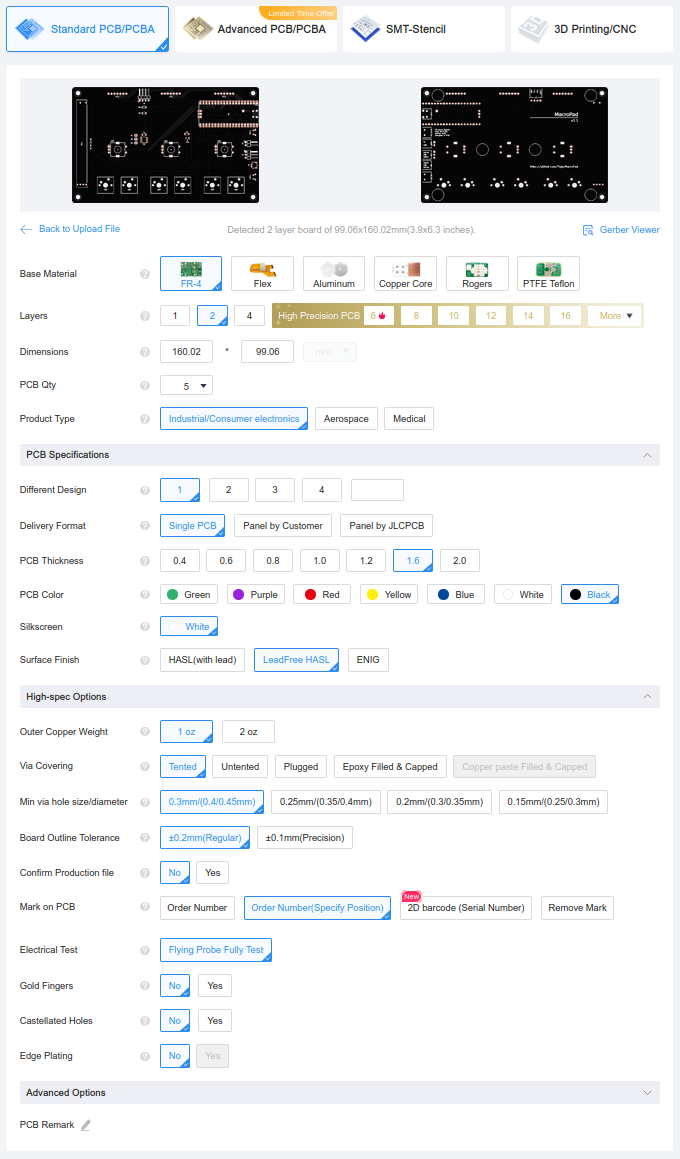
\includegraphics[scale=0.5]{Images/PcbOrderingExample.png}
\caption{Example for Ordering PCBs}
\label{fig:pcb_ordering_example}
\end{figure}

\subsubsection{Electronic (and Other) Components}
Figure \ref{fig:bom} is the Bill of Materials (BOM).
It contains product codes for a popular European, American, and Chinese retailer each. Again, this is just to give you an example and does not constitute an endorsement of those sellers. There are myriads of alternatives, many of which might be cheaper or have better availability in your country.

\begin{landscape}
\begin{figure}[htb]
\centering
\begin{longtable}{|l|l|l|c|l|l|l|}\hline
\textbf{Ref}&\textbf{Component}&\textbf{Value}&\textbf{Qty}&\textbf{reichelt.de}&\textbf{mouser.com}&\textbf{AliExpress}\cr\hline\hline
\multicolumn{7}{|c|}{\emph{Necessary Components}}\cr\hline
C2&Ceramic Capacitor&1206, 100nF&1&WAL 1206B104K500&GRM033Z71C104KE14D&\cr\hline
DS1..3&OLED Display&1.3'', SPI (7-pin), SH1106&3&&&\href{https://www.aliexpress.com/item/1005006127524245.html}{Link}\cr\hline
R1,R2&Resistor&1206, 4.7k\textOmega, $\nicefrac{1}{4}$W&2&WAL WR12X4701FTL&279-CRG1206F4K7/10&\cr\hline
\multirow{2}{*}{RV1}&Slide potentiometer&Stereo, linear, 75mm, 10k\textOmega&1&RS60112-LIN10K&688-RS60112A600N&\cr\cline{2-7}
&Knob&&1&KNOPF 4X1,2SW&&\cr\hline
\multirow{2}{*}{SW1..6}&Mechanical switch&Cherry MX Brown&6&CHERRY MX1A-G1NW&540-MX1A-G1NW&\href{https://www.aliexpress.com/item/1005005448524292.html}{Link}\cr\cline{2-7}
&Key caps&For Cherry MX, black&6&&&\href{https://www.aliexpress.com/item/1005006790237962.html}{Link}\cr\hline
\multirow{2}{*}{SW7..9}&Rotary Encoder&15mm shaft length, D-type&3&STEC12E08&858-EN11-VSM1AF15&\href{https://www.aliexpress.com/item/1005005983134515.html}{Link}\cr\cline{2-7}
&Knob&32mm, aluminium, black&3&&&\href{https://www.aliexpress.com/item/1005002272457890.html}{Link}\cr\hline
SW10&Micro switch&2x4x3.5mm, right angle&1&&&\href{https://www.aliexpress.com/item/32873390410.html}{Link}\cr\hline
U1&Raspberry Pi Pico&&1&RASP PI PICO&358-SC0915&\href{https://www.aliexpress.com/item/1005006800440665.html}{Link}\cr\hline
U2&EEPROM&24C512, 64kByte, SOP-8&1&&556-AT24C512C-SSHM-B&\cr\hline
&Rubber/Silicone Feet&Adhesive, $\diameter$11mm $\times$ 5mm&4..6&3M SJ5003 BLACK&517-SJ-5003BK&\href{https://www.aliexpress.com/item/1005005994012506.html}{Link}\cr\hline
&Stand-offs&Male/female, M3, 8mm, black&4&VT DA 8MM&710-971080365&\multirow{2}{*}{\href{https://www.aliexpress.com/item/1005006422618943.html}{Link}}\cr\cline{1-6}
&Bolts and nuts&M3, black&4&&&\cr\hline
&USB cable&Micro or type C, depending on U1&1&&&\cr\hline
\hline\multicolumn{7}{|c|}{\emph{Optional Components}}\cr\hline
C1&Ceramic Capacitor&1206, 100nF&1&WAL 1206B104K500&GRM033Z71C104KE14D&\cr\hline
J1&Pin Header&2.54mm, 1 row, 3 pins&1&SL 1X40W 2,54&538-22-28-6030&\cr\hline
J2&Connector&JST SH SM03B-SRSS-TB&1&&306-SM03BSRSSTBLFSNP&\href{https://de.aliexpress.com/item/1005006027334406.html}{Link}\cr\hline
J3&Pin Header&2.54mm, 1 row, 2 pins&1&SL 1X40W 2,54&538-22-28-6021&\cr\hline
J4&Pin Header&2.54mm, 1 row, 4 pins&1&SL 1X40W 2,54&538-22-28-6040&\cr\hline
SW11&Micro switch&2x4x3.5mm, right angle&1&&&\href{https://www.aliexpress.com/item/32873390410.html}{Link}\cr\hline
U3&Voltage reference&LM4040, 3.0V, SOT-23&1&LM 4040 CIM3-3.0&926-LM4040CIM330NOPB&\cr\hline
\end{longtable}
\caption{Bill of Materials}
\label{fig:bom}
\end{figure}
\end{landscape}

\paragraph{Necessary Components}
The OLED displays don't have a real name or product number but you'll find plenty of them for cheap on marketplaces like eBay or AliExpress. Make sure to get the SPI variant (7 pins) and not the I²C variant (4 pins).

The slide potentiometer is stereo (i.e.\ two mechanically connected potentiometers in one, typically used in audio devices) even though we're only using one. We found that the stereo ones are more widely available and often cheaper than the mono variant. We don't recommend buying the potentiometer from less reputable sources since there are massive differences in quality. 

For the Raspberry Pi Pico you can use the original one or a clone with the same form factor. The latter might differ in the quality of the flash memory and the voltage regulator, but the microcontroller itself is always the same RP2040 chip.\\
The one big advantage of clones is that they are available with a USB-C connector, whereas the original Pico only comes with Micro USB.\\
Other than some issues when flashing via SWD (see Section \ref{sec:fwflash}) -- which you don't need to do -- you won't notice any difference between the two.

\paragraph{Optional Components}
U3 and C1 can be used to stabilize the reference voltage for the Pico's analogue-to-digital converter (ADC) which reads the slide potentiometer.
Under normal circumstances this shouldn't be necessary. Note that the LM4040 will require approximately 1.5mA all the time which might violate the USB suspend current limit.

J1..4 and SW11 are useful if you want to work on the firmware but they are not required for normal operation.
J3 is a UART connector where the Pico prints debug messages.
J1 is an SWD connector for easier flashing and debugging. J2 is an alternative to J1 for use with the Raspberry Pi Debug Probe.
J4 is an I²C connector where you can monitor the traffic between the Pico and the EEPROM (or connect other I²C devices).
SW11 is the Pico's reset button.

\subsection{Soldering}
Through-hole components are the easiest to solder: just stick them into the PCB, then solder them in from the back. Make sure the soldering iron heats both the component's leg and the PCB's pad. If the solder doesn't stick to both, apply some flux. 

Surface-mount components are slightly more difficult, mostly due to their size. First, apply some flux to the pads. Heat one pad and apply a small amount of solder. Then, while heating the solder on the pad with one hand, slider the component into its place with the other. At this time, the solder joint doesn't have to be nice, its only purpose is to hold the component in its correct place. Once you've achieved that, solder the other pad(s). After that, you can re-do the first solder joint if necessary. 
If the solder bridges adjacent pins, add some flux and reheat them. If this doesn't fix it, use wick to remove surplus solder. 

The recommended order for soldering is first the small components (R1, R2, C2, U2, SW10), then the Pi Pico (U1), then the rotary encoders, switches, and slider (SW1..9, RV1). 

Make sure the EEPROM (U2) is in the correct orientation. The chip has a small indent in one corner which has to align with the marking on the PCB.\\
Try to position the Pi Pico (U1) as precisely as possible. It is important that the test pad on the back line up with the through-hole in the PCB (this connects the BOOTSEL button). Put a small amount of solder in the hole to connect it. 

After that, check all connection using the continuity test mode of your multimeter. Once the displays are soldered, many solder joints become inaccessible. 

Insert the displays loosely. Mount the front plate and turn the device upside down. Shake gently so that the displays come to lie flush against the front plate, then solder them in from the back side. 

Figure \ref{fig:assembly} shows the finished PCB. 

\begin{figure}[htb]
\centering
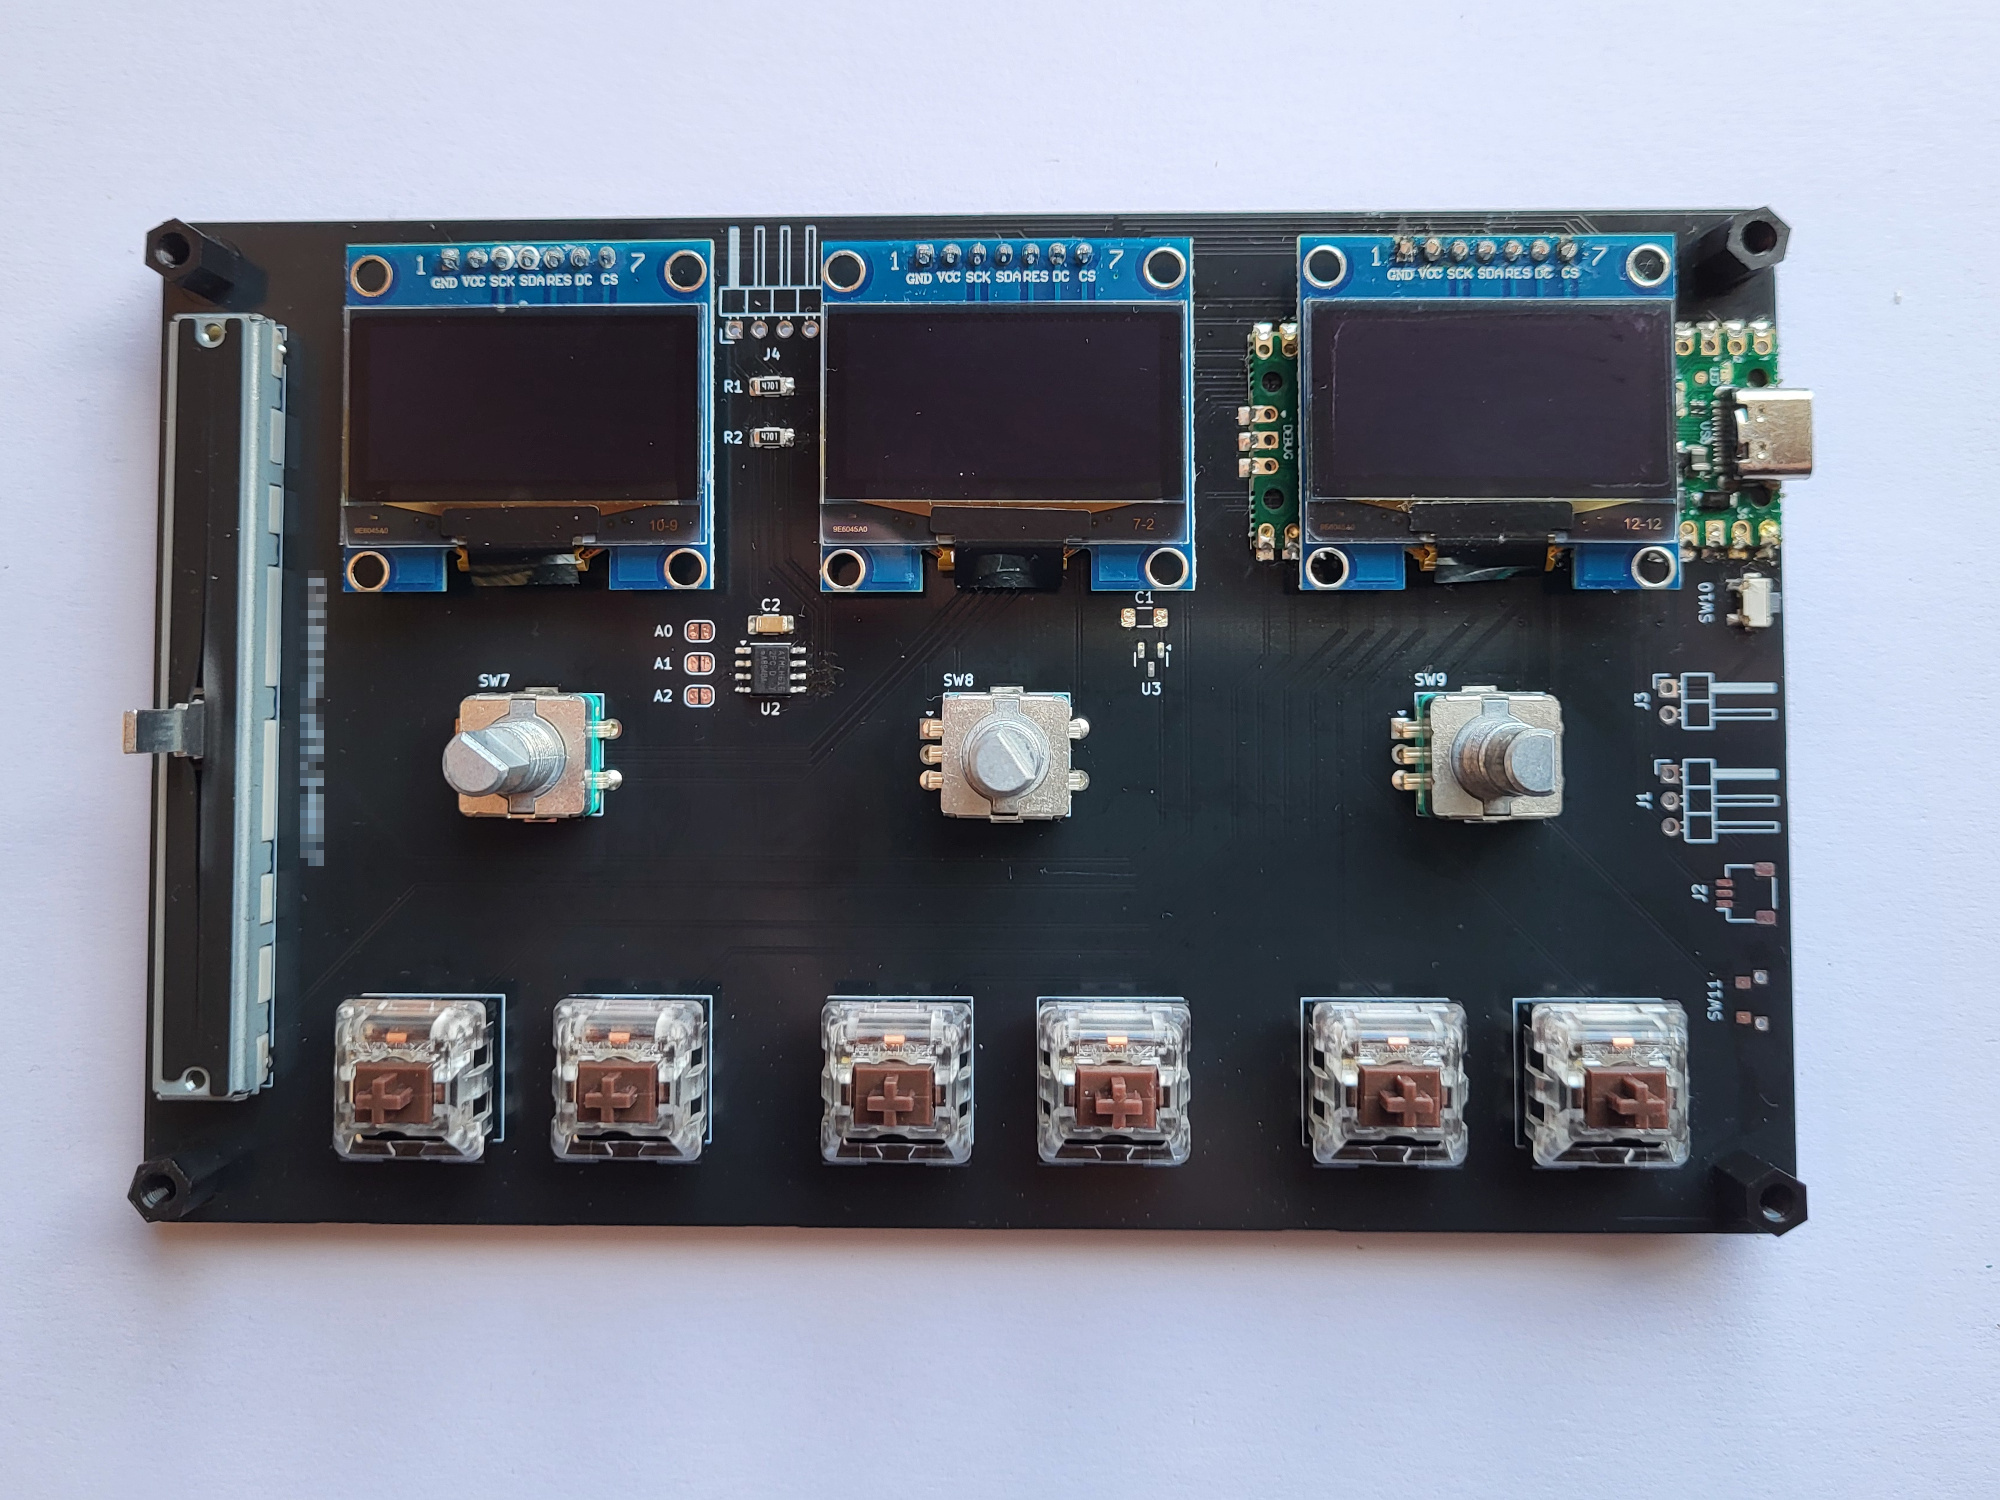
\includegraphics[width=\textwidth]{Images/Assembly.jpg}
\caption{Assembly of the Back PCB}
\label{fig:assembly}
\end{figure}

Finally, put on the keycaps and knobs. When mounting the knobs onto the rotary encoders, make sure they can be pressed without touching the front plate. 

\section{Firmware}
The firmware is the code that runs on MacroPad's Raspberry Pi Pico microcontroller.

\subsection{Building the Firmware}\label{sec:fwcompile}
\begin{note}
This section is only relevant if you want to compile the firmware yourself from source code.
Otherwise you can just use the finished firmware file (\file{MacroPad.uf2}) from the GitHub repository.
\end{note}

You need to have the following tools and libraries installed:
\begin{itemize}
\item Git: You have already installed this in Section \ref{sec:gitclone}.
\item CMake: The build system used for compiling everything in this repository.
\item C++ Toolchain: Cross compiler and related tools.
\item (Optional) Doxygen: Create documentation for all the classes and functions.
\end{itemize}

If you are on a Debian-based Linux (e.g.\ Ubuntu), you can just install everything with the following command:
\begin{lstlisting}[language=bash]
sudo apt-get install git cmake gcc-arm-none-eabi libnewlib-arm-none-eabi build-essential g++ libstdc++-arm-none-eabi-newlib doxygen
\end{lstlisting}

Open a terminal and change into the \file{Firmware} subdirectory of the downloaded repository. Create a folder named build and change into it:
\begin{lstlisting}[language=bash]
mkdir build
cd build
\end{lstlisting}
Run CMake, then make:
\begin{lstlisting}[language=bash]
cmake ..
make
\end{lstlisting}
After that, you can find the MacroPad.uf2 firmware file inside the build folder.

\subsection{Flashing the Firmware}\label{sec:fwflash}
This section explains how to flash the compiled firmware onto the device via SWD using the \href{https://www.raspberrypi.com/documentation/microcontrollers/debug-probe.html}{Raspberry Pi Debug Probe}.

\begin{note}
Unless you need to flash very often (e.g.\ during debugging), USB is the easier way to go.
Please refer to the User's Guide for how to flash the firmware onto the device via USB.
\end{note}

\subsubsection{Connecting the Debug Probe}
On the Debug Probe, use the connector labelled ``D''. The probe comes with a JST-to-JST as well as a JST-to-female cable. You can use either, depending on which one of connectors J1 and J2 you've soldered. In case of J1, the orange wire goes into SWCLK, the black wire into GND, and the yellow wire into SWDIO.

If you're connecting via J2, you can use the JST-to-female cable instead to hook up MacroPad's UART debug output to the probe's ``U'' connector. The black wire goes to GND and the yellow wire to TX.
The UART settings are 115200 baud, 8N1, and flow control enabled. 

\subsubsection{OpenOCD}
Download and install \href{https://openocd.org/}{OpenOCD} from the website or via your system's package manager. 

The command for flashing is included in the \file{CMakeLists.txt} file. All you need to do is run \lstinline[language=bash]{make flash} from the \file{build} directory. 

\begin{note}
For some reason, OpenOCD does not fully reset both cores of the Pico after flashing. You have to manually press the reset button or disconnect and reconnect the USB cable.
\end{note}

\subsubsection{Pi Pico Clones with Different Flash Chips}
Many clones of the Pi Pico come with different (probably cheaper) on-board flash chips than the original.
While OpenOCD is usually capable of flashing onto these chips, it uses an internal white list which your flash might not be on.
In this case, you will see an error that looks something like this:
\begin{lstlisting}[language=bash]
Error: Unknown flash device (ID 0x00184068)
\end{lstlisting}

Note down the ID from the error message, then perform the following steps to create a patched version of OpenOCD\footnote{Thanks to \href{https://forums.raspberrypi.com/viewtopic.php?t=359245}{this forum thread} for the idea.}:
\begin{enumerate}
\item Uninstall a previously installed OpenOCD.
\item Download the code from the OpenOCD GitHub repository, then change into the directory:
\begin{lstlisting}[language=bash]
git clone https://github.com/raspberrypi/openocd.git --branch rp2040-v0.12.0 --depth=1
cd openocd
\end{lstlisting}
\item Edit src/flash/nor/spi.c and add an entry to the \lstinline[language=C]{flash_devices[]} array, for example:
\begin{lstlisting}[language=C]
FLASH_ID("Unknown", 0x03, 0xeb, 0x02, 0xd8, 0xc7, 0x00184068, 0x100, 0x10000, 0x1000000),
\end{lstlisting}
Most of the values you can just copy from existing entries, but two are important:
In the seventh column, enter the device ID that you noted down earlier.
In the last column, enter the flash size in bytes (e.g.\ 16 megabytes is $2^{24}$ bytes which is 0x1000000 in hexadecimal).
\item Compile and install the modified OpenOCD:
\begin{lstlisting}[language=bash]
./bootstrap
./configure
make
sudo make install
\end{lstlisting}
\end{enumerate}

\iffalse
# How to create the new entry:
# This forum post mentions the technique and gives an exampe for a specific (but
# different) flash chip: https://forums.raspberrypi.com/viewtopic.php?t=359245
# FLASH_ID("pu p32q32", 0x03, 0xeb, 0x02, 0xd8, 0xc7, 0x00156085, 0x100, 0x10000, 0x400000),
#
# The RP2040 datasheet puts pretty strict limits on the kinds of flash chips it
# can use as program memory. This suggests that the parameters should be pretty
# much the same as those of supported chips that are found on the original Pico.
# So far, taking the entry above and only changing the device id (7th column)
# and the size in bytes (last column) has worked.
\fi

\section{Settings App}
MacroPad comes with an application that allows you to change the settings. This application is available for Linux and Windows. You can download it from the GitHub repository.

\begin{note}
The app will probably also compile for Mac, but this has not been tested.
\end{note}

It is also possible to compile the app yourself from source code. Two libraries are required: \href{https://github.com/libusb/hidapi}{HIDAPI} (for communication via USB) and \href{https://www.wxwidgets.org/}{wxWidgets} (for the graphical user interface). You also need CMake and a C++ compiler, both of which you have already install in Section \ref{sec:fwcompile}. 

\subsection{Building on Linux}
Install the necessary libraries:
\begin{lstlisting}[language=bash]
sudo apt-get install libwsgtk3.2-dev libhidapi-dev
\end{lstlisting}

In a terminal, go to the \file{Software} subdirectory of the downloaded repository, then run: 
\begin{lstlisting}[language=bash]
mkdir build
cd build
cmake ..
make
\end{lstlisting}

After that, you will find the executables called \file{MacroPad} and \file{macropad-cli} in the \file{build} directory. 

\subsection{Building on Windows}
TODO

\section{Miscellaneous}
\subsection{USB Vendor ID and Product ID}
USB devices need a Vendor ID (VID) and Product ID (PID) to be identified by the host. VIDs and PIDs are 4-digit hexadecimal numbers. Commercial manufacturers licence their VID from the \href{https://www.usb.org/getting-vendor-id}{USB Implementers Forum (USB-IF)}.
As a hobbyist project, MacroPad does not have a VID or PID. However, for private use, no one prevents you from just using a made-up VID/PID combination (ideally one that is not used by another device).
You can specify the VID/PID in the usb\_descriptors.h file. After doing so, you need to recompile both the firmware and the Settings App.

\subsection{Key Rollover}
Key rollover describes the ability of a keyboard to register (and report to the host) multiple keys being held down at the same time. Pretty much all USB keyboards support at least 6-key rollover (6KRO). Higher-end ones even allow arbitrarily high $n$-key rollover (NKRO). Modifier keys (shift, control, alt, windows) typically do not count towards the KRO number.

There is a common misconception that USB keyboards are limited to 6KRO. This is false, albeit with a kernel of truth: USB HID\footnote{Human Interface Device}-class devices send data to the host (the computer) at regular intervals in data packages called ``reports''. The format of these reports (and as a consequence the maximum possible number of concurrently pressed keys) is not fixed. Instead, each device specifies the exact format via a ``report descriptor''. While this allows for incredible flexibility, it also makes HID drivers on the host side (those usually come with the operating system) quite complex: The driver has to read the report descriptor and from it generate a bespoke parser for each device. Not all systems have the ressources to do that. In particular, older BIOSes tend not to implement a full USB HID driver. For this reason, a special type of USB HID device was defined. These so called ``boot-protocol keyboards'' have a fixed report descriptor which only allows 6KRO.

On the hardware level, MacroPad has no limitations regarding key rollover. All input controls are wired separately to the microcontroller, thanks to the relatively low number of switches and knobs. There is no matrix involved which makes eliminates any kind of ghosting.

On the software side, things become more interesting. Keep in mind that MacroPad is not a standard keyboard where each switch corresponds to one key being sent to the host. Instead, all input controls are freely programmable. In theory, you could configure a switch to act as if the whole alphabet had been pressed. In other words, the number of physical keys has nothing to do with how many keys are reported to the host.
MacroPad is capable of emulating a boot-protocol keyboard (with 6KRO) but it can also use the normal report protocol, in which case it has 16KRO by default. It is the host that chooses which protocol to use.

While the boot protocol's 6KRO is fixed, the 16KRO can be changed if you need higher rollover: When compiling the firmware, you can pass a flag setting a specific KRO value, for example:
\begin{lstlisting}[language=bash]
cmake -DKRO=20 ..
\end{lstlisting}
Note that higher values result in longer reports, eating more of the USB connection's bandwidth. Do not go beyond 60 otherwise you risk exceeding the size of a USB package. 

\end{document}
